% $Header: /cvsroot/latex-beamer/latex-beamer/solutions/generic-talks/generic-ornate-15min-45min.en.tex,v 1.5 2007/01/28 20:48:23 tantau Exp $

\documentclass[12pt]{beamer}
%\documentclass[12pt,handout]{beamer}

% This file is a solution template for:

% - Giving a talk on some subject.
% - The talk is between 15min and 45min long.
% - Style is ornate.



% Copyright 2004 by Till Tantau <tantau@users.sourceforge.net>.
%
% In principle, this file can be redistributed and/or modified under
% the terms of the GNU Public License, version 2.
%
% However, this file is supposed to be a template to be modified
% for your own needs. For this reason, if you use this file as a
% template and not specifically distribute it as part of a another
% package/program, I grant the extra permission to freely copy and
% modify this file as you see fit and even to delete this copyright
% notice.


\mode<presentation>
{
  \usetheme{default}
  % or ...

  \setbeamercovered{transparent}
  % or whatever (possibly just delete it)
}
\setbeamertemplate{navigation symbols}{}%remove navigation symbols


\usepackage[english]{babel}
% or whatever

\usepackage[latin1]{inputenc}
% or whatever

\usepackage{times}
\usepackage{sansmathfonts}
\usepackage[T1]{fontenc}
% Or whatever. Note that the encoding and the font should match. If T1
% does not look nice, try deleting the line with the fontenc.


\title%[Short Paper Title] % (optional, use only with long paper titles)
{}

\subtitle
{} % (optional)

\author%[Author, Another] (optional, use only with lots of authors)
{Ben Holder}%{F.~Author\inst{1} \and S.~Another\inst{2}}
% - Use the \inst{?} command only if the authors have different
%   affiliation.

%\institute[Universities of Somewhere and Elsewhere] % (optional, but mostly needed)
%{
%  \inst{1}%
%  Department of Computer Science\\
%  University of Somewhere
%  \and
%  \inst{2}%
%  Department of Theoretical Philosophy\\
%  University of Elsewhere}
%% - Use the \inst command only if there are several affiliations.
%% - Keep it simple, no one is interested in your street address.

\date%[Short Occasion] % (optional)
{}

\subject{Talks}
% This is only inserted into the PDF information catalog. Can be left
% out.



% If you have a file called "university-logo-filename.xxx", where xxx
% is a graphic format that can be processed by latex or pdflatex,
% resp., then you can add a logo as follows:

% \pgfdeclareimage[height=0.5cm]{university-logo}{university-logo-filename}
% \logo{\pgfuseimage{university-logo}}



% Delete this, if you do not want the table of contents to pop up at
% the beginning of each subsection:
%\AtBeginSubsection[]
%{
%  \begin{frame}<beamer>{Outline}
%    \tableofcontents[currentsection,currentsubsection]
%  \end{frame}
%}


% If you wish to uncover everything in a step-wise fashion, uncomment
% the following command:

%\beamerdefaultoverlayspecification{<+->}

\usepackage{enumerate}
\usepackage{amsmath}
\usepackage{amssymb}
\usepackage[amssymb]{SIunits}
\usepackage{url}
\usepackage{hyperref}
\usepackage[normalem]{ulem}


\setbeamercovered{invisible}

\hypersetup{
    colorlinks=true,     % false: boxed links; true: colored links
    linkcolor=red,       % color of internal links
    citecolor=blue,      % color of links to bibliography
    filecolor=blue,      % color of file links
    urlcolor=blue        % color of external links
}


\begin{document}

%\begin{frame}
%  \titlepage
%\end{frame}

%%%%%%%%%%%%%%%%%%%%%%%%%%%%%%%%%%%%%%
\begin{frame}{Announcements}
	%
	\begin{itemize}
	\addtolength{\itemsep}{0.5\baselineskip}
	\item Any questions/issues?
	\item \underline{Schedule}:
		%
		\begin{itemize}
		\item[]{\bf Today (Follow-up)}: Question 2 from ``Forcing and Timescales'' discussion --- Exponential Growth and Doubling
		\item[]{\bf Today (New)}: Modeling and forecast of climate change
		\item[]{\bf Tomorrow (Lab)}: Computational Modeling (web app)
		\item[]{\bf Thursday (Discussion)}: More Computational Modeling
		\item[] {\bf Next Week}: Oceans and Ice
		\end{itemize}
		%
	\end{itemize}

\end{frame}
%%%%%%%%%%%%%%%%%%%%%%%%%%%%%%%%%%%%%%
\begin{frame}{Today's Reading Quiz (3 min)}


%	
%\vspace{1cm}
%
%On your own sheet of paper\ldots
%
%\vspace{0.5cm}
%
%{\bf Briefly explain \underline{radiative forcing}. What are its units and why?  How does it affect temperature of the Earth? Can you give one example?}
%\vspace{0.5cm}
%
%Turn in to Blackboard as scanned pdf (or image is fine).


No reading for today, but please prepare for tomorrow and Thursday by:
	%
	\begin{itemize}
	\item Reading Chapter 8 from Dessler (``Predictions of Future Climate Change'')
	\item Watching the \href{https://www.youtube.com/watch?v=4O-5fsVZaII}{tutorial video} for the climate simulator \href{https://en-roads.climateinteractive.org/}{{\bf EN-ROADS}} (find link on ``Weekly Reading Assignments'' page)
	\end{itemize}
	

\end{frame}
%%%%%%%%%%%%%%%%%%%%%%%%%%%%%%%%%%%%%%
\begin{frame}{Final Poster Project}

\begin{itemize}
\item Choose a topic that is interesting to you and make a poster to present (5min) to the class during our final exam period (Thurs, Dec 11, 10am).
\item Work on your own or with a partner.
\item Think of it as a Discussion/Lab/Lecture that you create, explaining some topic to yourself and us.
\item {\bf Talk to me by Thanksgiving (Tues Nov 25)} to verify your project topic ({\bf worth one Discussion assignment}).
\item In the last week of class you will have time (lecture and discussion) to work on your final poster project. 
	
\end{itemize}


\end{frame}
%%%%%%%%%%%%%%%%%%%%%%%%%%%%%%%%%%%%%%
\begin{frame}{Exponential Growth of $\text{CO}_2$ concentration}


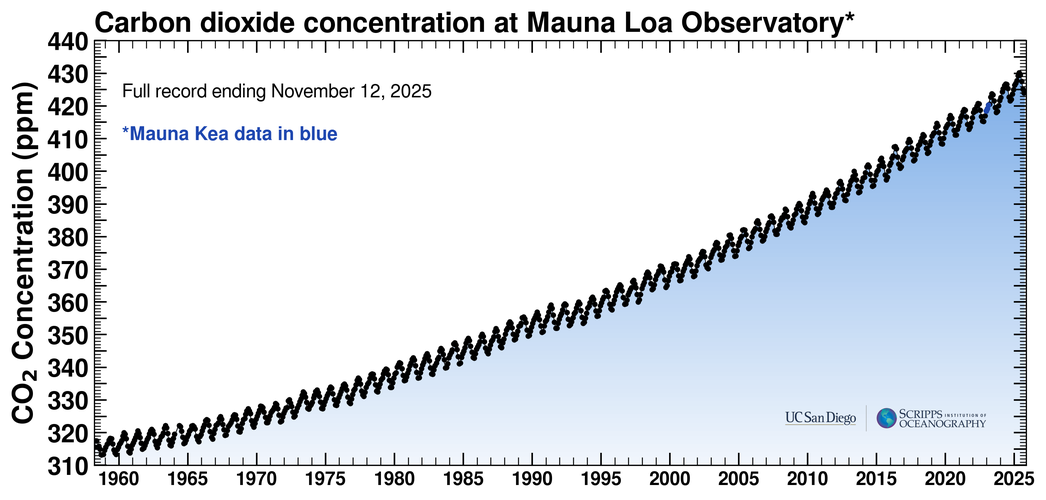
\includegraphics[width=\textwidth]{images/keeling-curve_mlo-full-record_2025-11-13.png}

\end{frame}
%%%%%%%%%%%%%%%%%%%%%%%%%%%%%%%%%%%%%%
\begin{frame}{$\text{CO}_2$ concentration on planetary timescales}


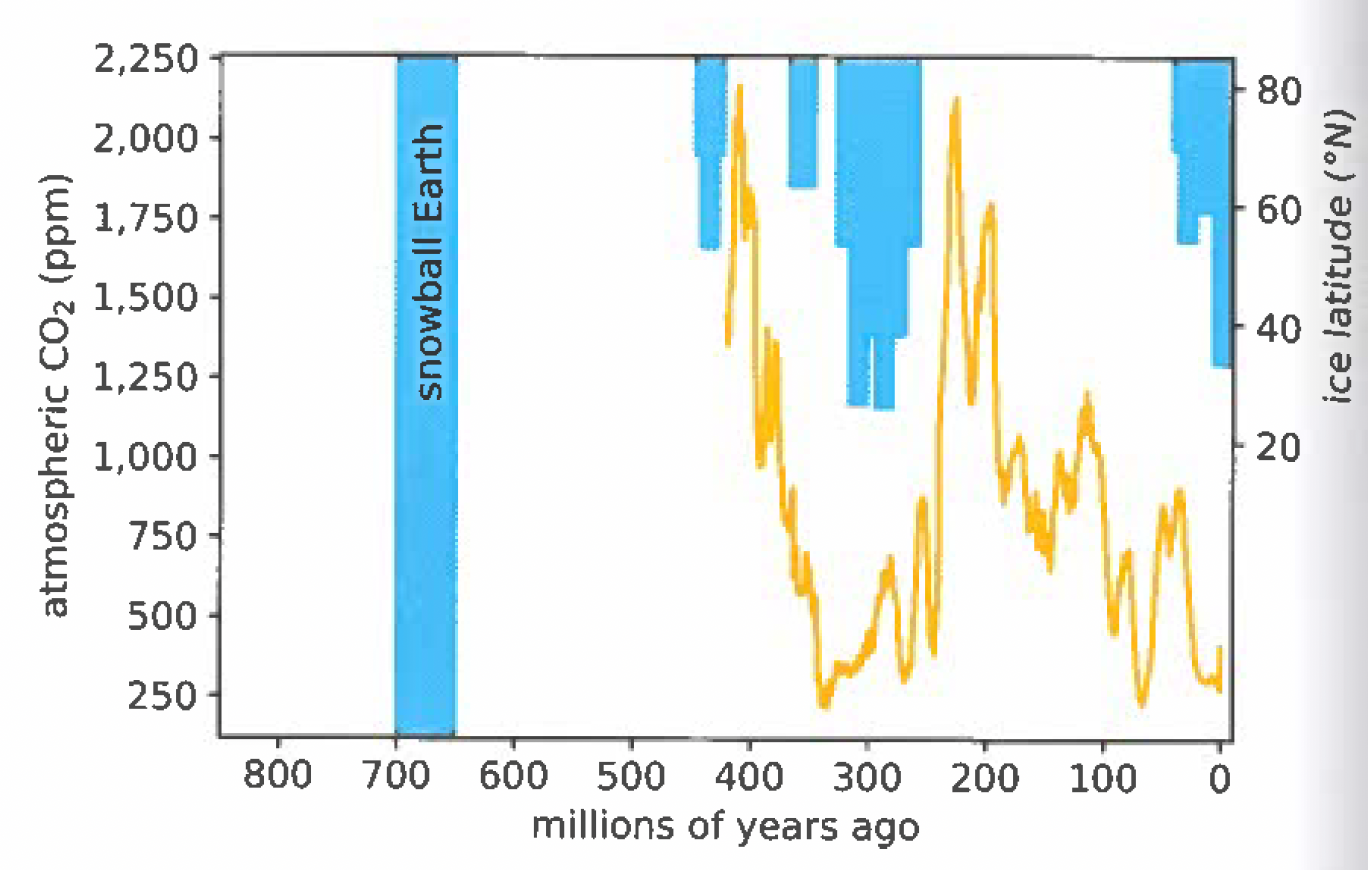
\includegraphics[width=\textwidth]{images/dessler_fig7-7.png}
{\tiny Dessler Fig 7.7}

\end{frame}
%%%%%%%%%%%%%%%%%%%%%%%%%%%%%%%%%%%%%%
\begin{frame}{$\text{CO}_2$ and temperature}


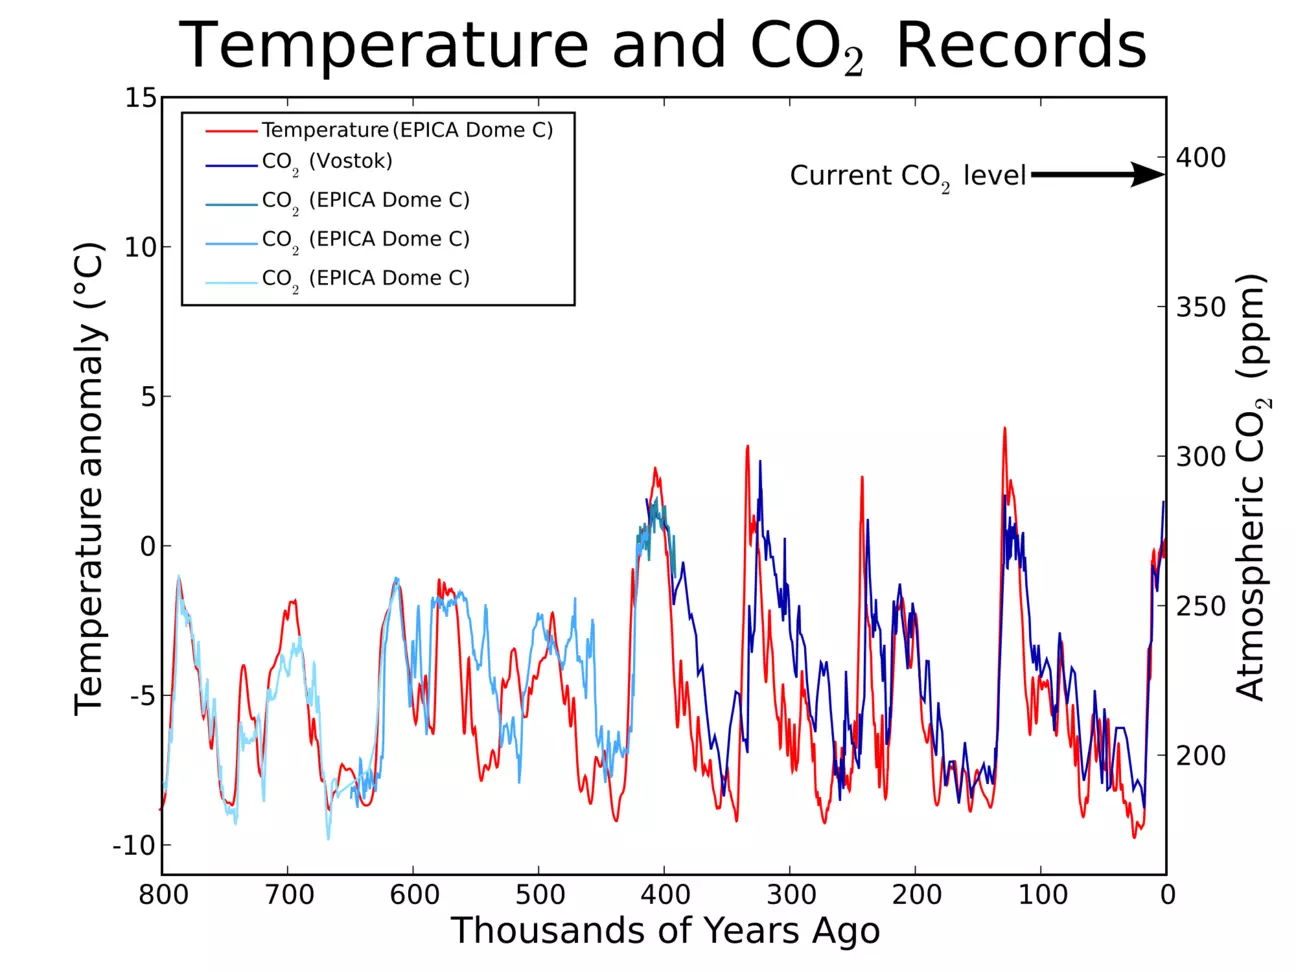
\includegraphics[width=\textwidth]{images/temperature-and-co2-800ky_carleton-serc.png}
{\tiny Carleton College SERC}

\end{frame}
%%%%%%%%%%%%%%%%%%%%%%%%%%%%%%%%%%%%%%
\begin{frame}{The last big temperature/$\text{CO}_2$ surge: PETM}


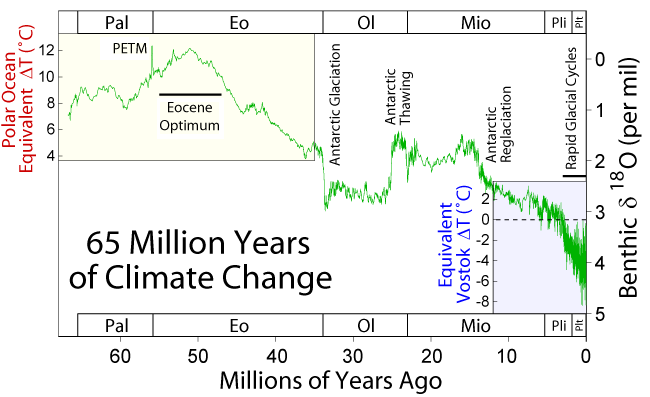
\includegraphics[width=\textwidth]{images/65_Myr_Climate_Change_wikimedia-rohde.png}
{\tiny Wikimedia (Rohde)}

\end{frame}
%%%%%%%%%%%%%%%%%%%%%%%%%%%%%%%%%%%%%%
\begin{frame}{PETM timescale}


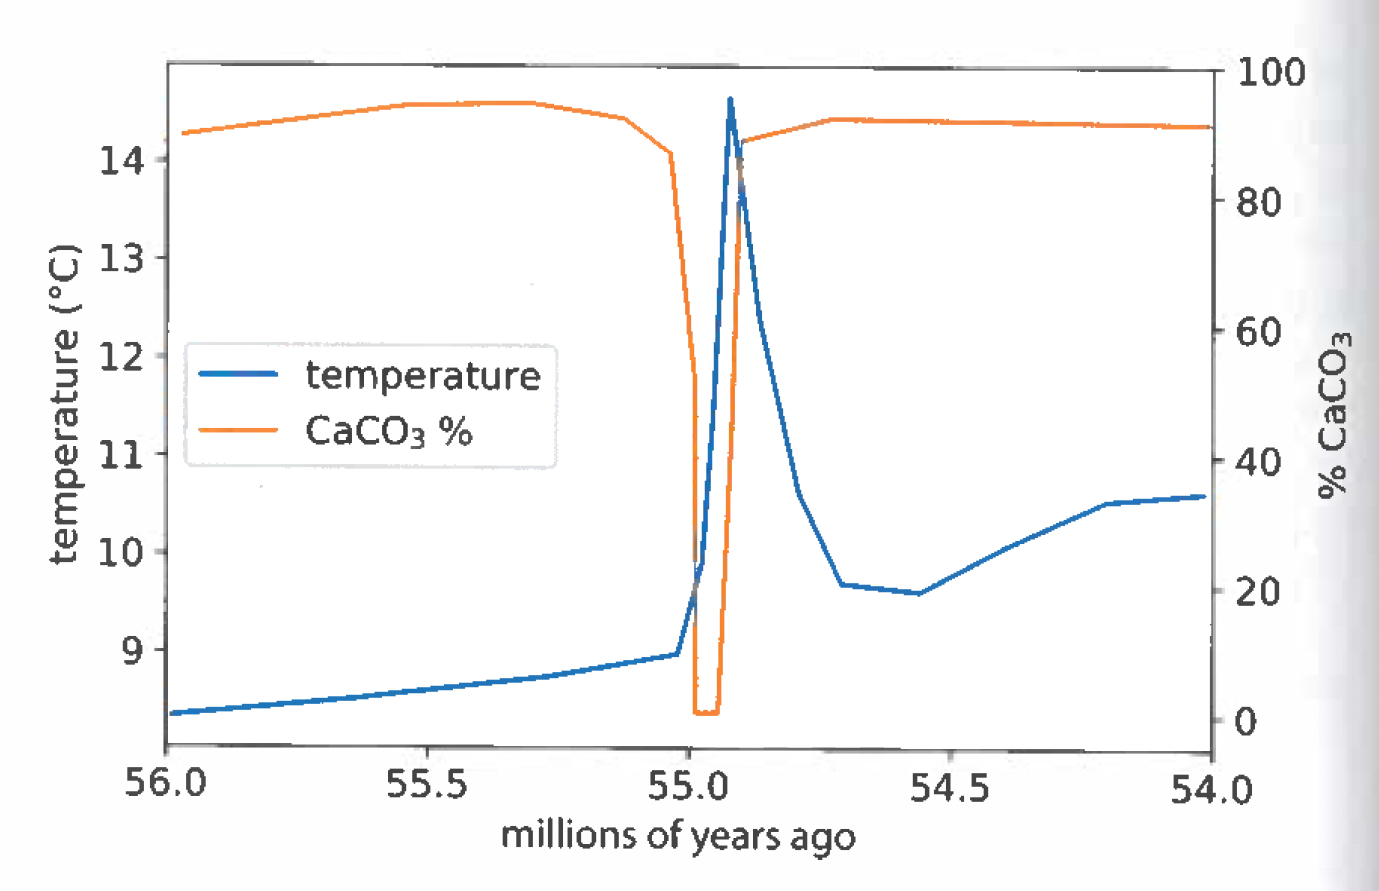
\includegraphics[width=\textwidth]{images/dessler_fig7-8.png}
{\tiny Dessler Fig 7.8}

\end{frame}
%%%%%%%%%%%%%%%%%%%%%%%%%%%%%%%%%%%%%%
\begin{frame}{PETM timescale}


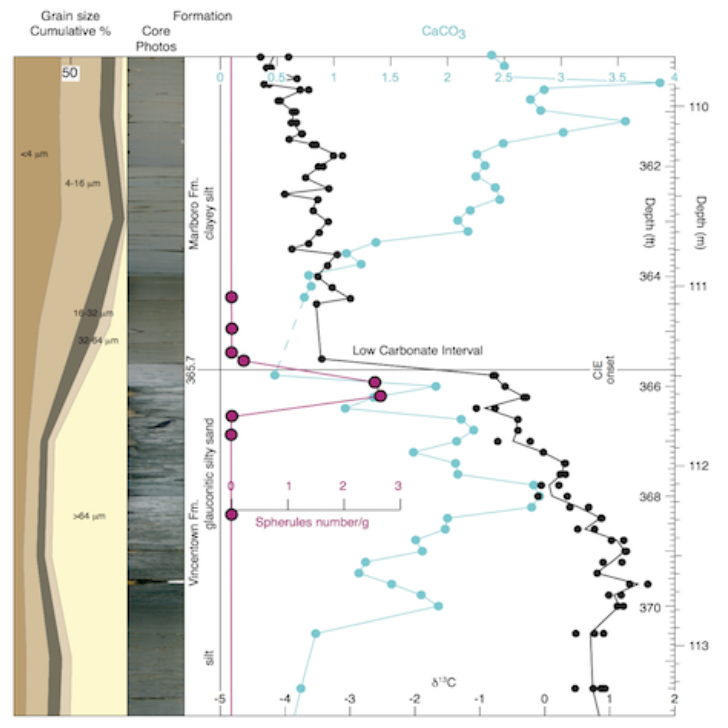
\includegraphics[width=0.75\textwidth]{images/PETM_Wilson_Lake.png}\\
{\tiny Rutgers, Marlboro Clay Project}

\end{frame}
%%%%%%%%%%%%%%%%%%%%%%%%%%%%%%%%%%%%%%
\begin{frame}{Timescales of contemporary climate change}


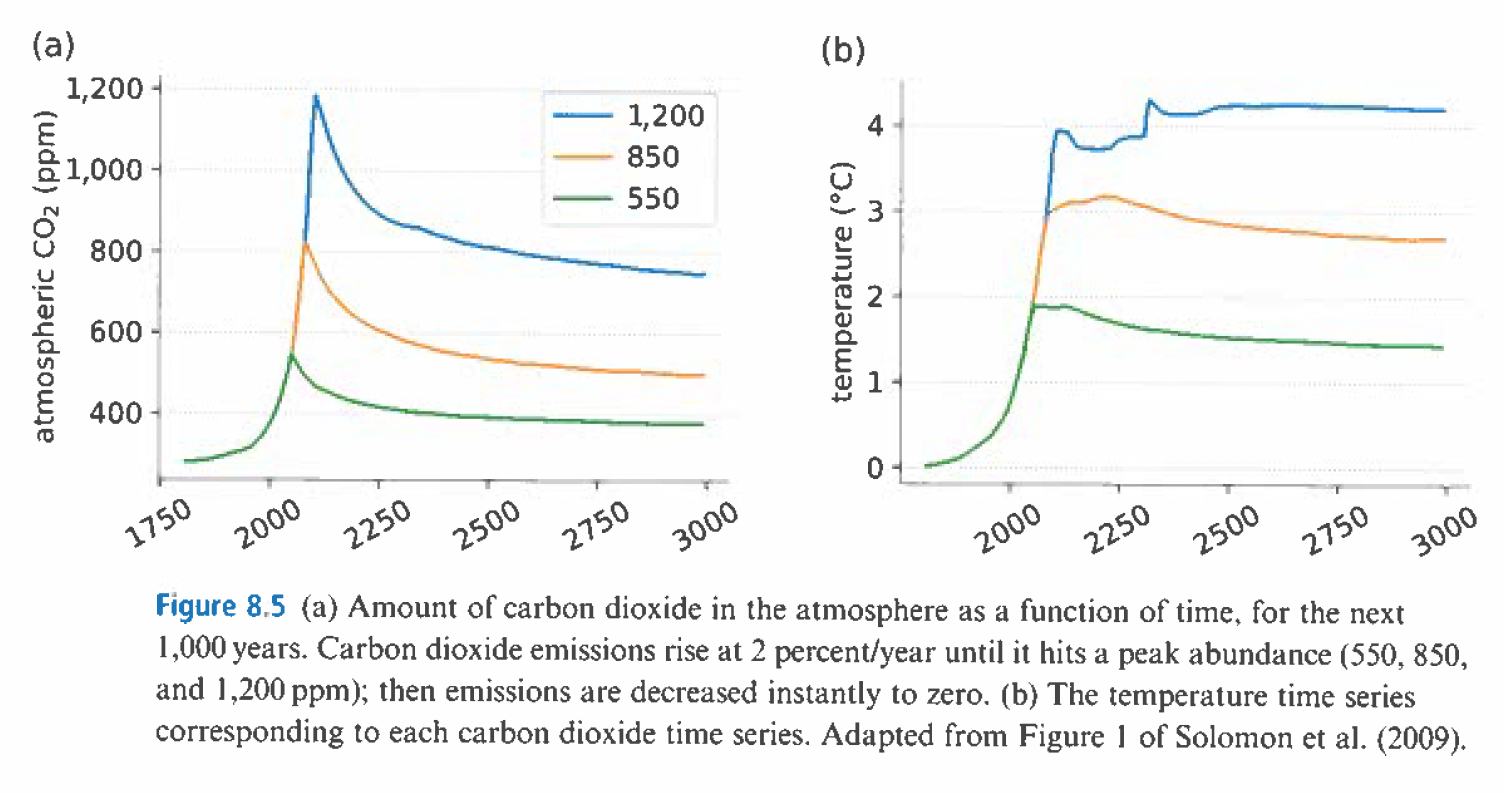
\includegraphics[width=\textwidth]{images/dessler_fig8-5.png}
{\tiny Dessler}

\end{frame}
%%%%%%%%%%%%%%%%%%%%%%%%%%%%%%%%%%%%%%





\end{document}
